% \section{Timestamps}
\label{sec:timestamps}

\subsection{Timestamps Generation in Attention-Encoder Decoder Models}

The extraction of precise timestamps from spoken words is a critical capability of modern Speech Recognition systems, essential for powering downstream applications such as timed subtitling and content retrieval. The methods for extracting timestamps from attention-based speech recognition models are diverse, ranging from post-processing techniques to architectural redesigns. Each approach represents a different trade-off between accuracy, computational overhead, and architectural complexity.

The architecture that we are working with in Canary-1B-v2 is an attention-based encoder-decoder (AED) system. In these models, alignment between audio frames and text tokens is handled during the decoding phase. This is primarily facilitated by the cross-attention mechanism, which produces a weight matrix representing the probabilistic correlation between each output token and every input audio frame. While these weights provide a "soft" alignment, they are prone to non-monotonicity, where the attention path can jump back and forth in time, leading to a certain degree of inherent unreliability or "fuzziness."

\subsubsection{Post-Processing with Dynamic Time Warping (DTW)}
To convert this soft, often non-monotonic alignment into precise, word-level boundaries, a robust post-processing algorithm like Dynamic Time Warping (DTW)\cite{DTWAlignment} is applied to the cross-attention matrix. DTW finds the optimal, non-linear alignment path between two sequences by computing a cumulative cost or score matrix. In this context, it aligns the sequence of output tokens with the sequence of input audio frames by finding the path of highest cumulative attention scores. This process effectively "hardens" the fuzzy attention into a clear, monotonic sequence of word boundaries, providing the start and end times for each word. A prominent example of this method is its use in third-party implementations\cite{lintoai2023whispertimestamped} for Whisper\cite{radford2023whisper} model, which natively provides only segment-level timestamps.

\subsubsection{Predictive Timestamp Generation}

A fundamentally different approach is to embed timestamp prediction directly into the AED model itself. In this setup, timestamping is reframed as a core predictive task rather than a post-processing step. Whisper \cite{radford2023whisper} first introduced this strategy by training on a corpus in which special frame-number tokens (e.g., \emph{<|0|>, <|1|>, …}) were inserted into transcriptions at segment boundaries. The Canary model \cite{canary1b-flash-timestamps} subsequently adopted and extended this approach by inserting the tokens at word boundaries. By learning to predict these tokens directly, the model incorporates an understanding of acoustic–temporal relationships into its core predictive capability.

This approach has distinct advantages, as it shifts the alignment burden to the model's training process. However, it also introduces new complexities:

\begin{itemize}
    \item \textbf{Data Curation:} The creation of a diverse and well-represented training corpus with accurate timestamp tokens requires significant computational resources and careful data curation.
    \item \textbf{Training Challenges:} The model must now learn an additional task, which can create balancing issues and requires a more carefully tuned training regimen to avoid negatively impacting transcription accuracy.
\end{itemize}


\subsubsection{Forced Alignment as a Standalone Method}

For many production and commercial applications\cite{whisperX}, the process of timestamping has been abstracted away into a service. Forced alignment, a method that takes an audio file and its corresponding transcript to generate timestamps, serves as a powerful standalone. 
Given the complexities and potential instability of relying solely on "soft" attention weights or multi-task learning for timestamps, we explored exactly the forced alignment method as a standalone approach for Canary-1B-v2. Unlike the methods above, it does not rely on the end-to-end model's internal alignment mechanism for timestamping.

For our purposes, the NeMo Forced Aligner (NFA)\cite{nfa} has proven to be an effective method for generating word and segment-level timestamps in \cite{canary1b-flash-timestamps}. This method has become the backbone for timestamp extraction in our system, used in conjunction with auxiliary Multilingual Parakeet CTC model.

\subsection{NeMo Forced Aligner (NFA)}

NeMo Forced Aligner (NFA) is a tool for generating token-, word-, and segment-level timestamps of speech in audio using CTC-based ASR models. Optionally, NFA can align ground truth text with the CTC-based ASR model decoder's log-probabilities. The alignment process uses Viterbi decoding to find the most probable alignment of given tokens based on log-probabilities from the CTC head.

\begin{figure}[htbp]
  \centering
  % Subfigure (a) on top
  \begin{subfigure}{\textwidth}
    \centering
    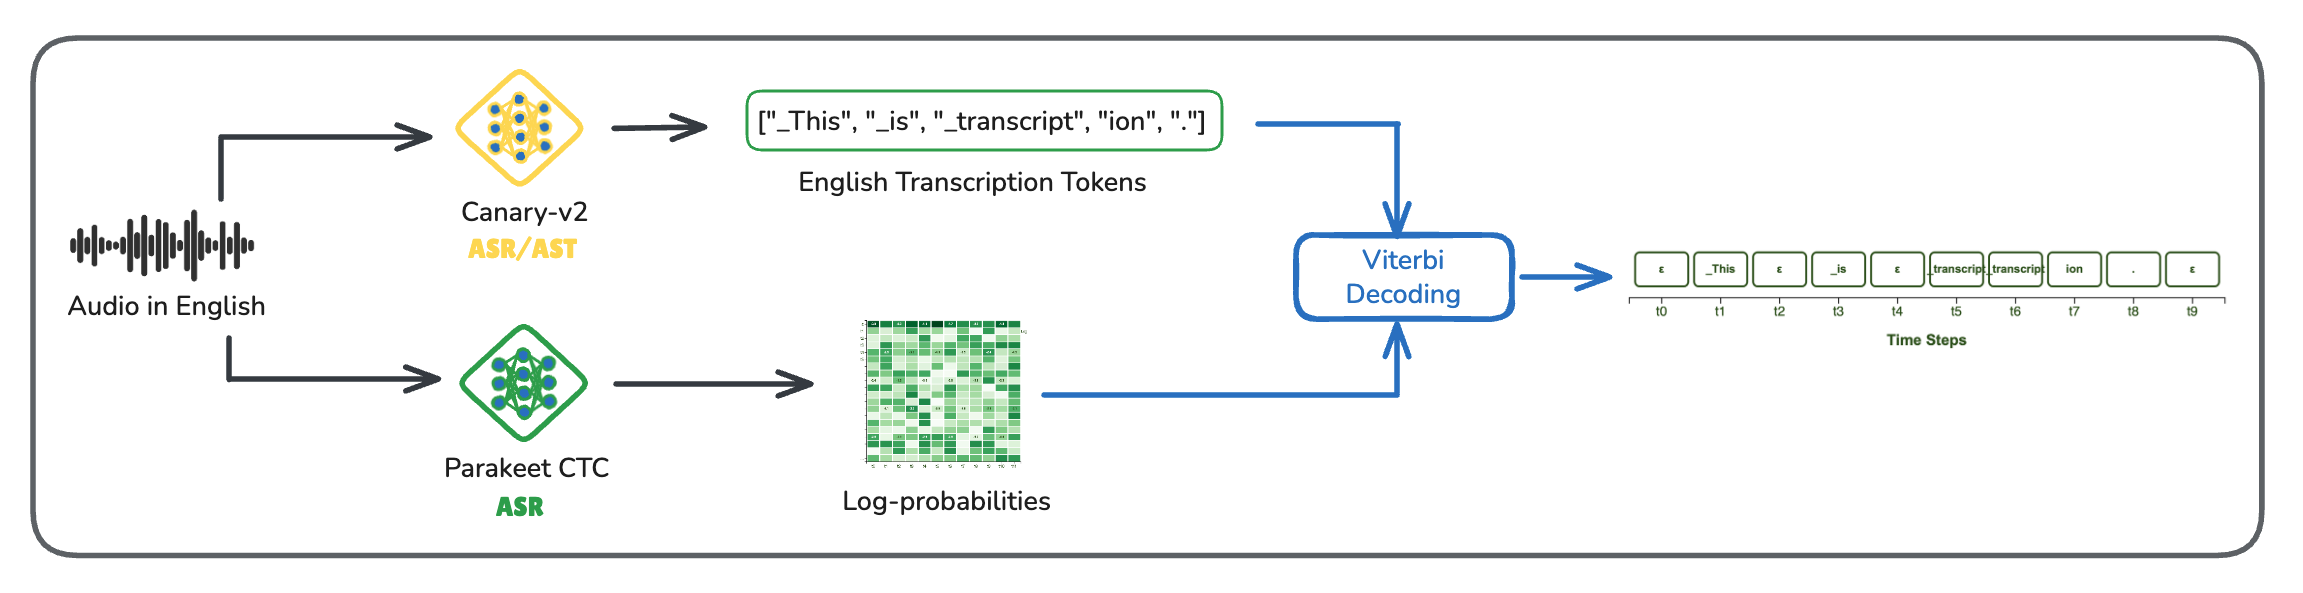
\includegraphics[width=0.95\linewidth]{images/nfa_a.png}
    \caption{Timestamps for ASR output.}
    \label{fig:canary-timestamps-asr}
  \end{subfigure}

  \vspace{1em} % optional vertical space between (a) and (b)

  % Subfigure (b) below
  \begin{subfigure}{\textwidth}
    \centering
    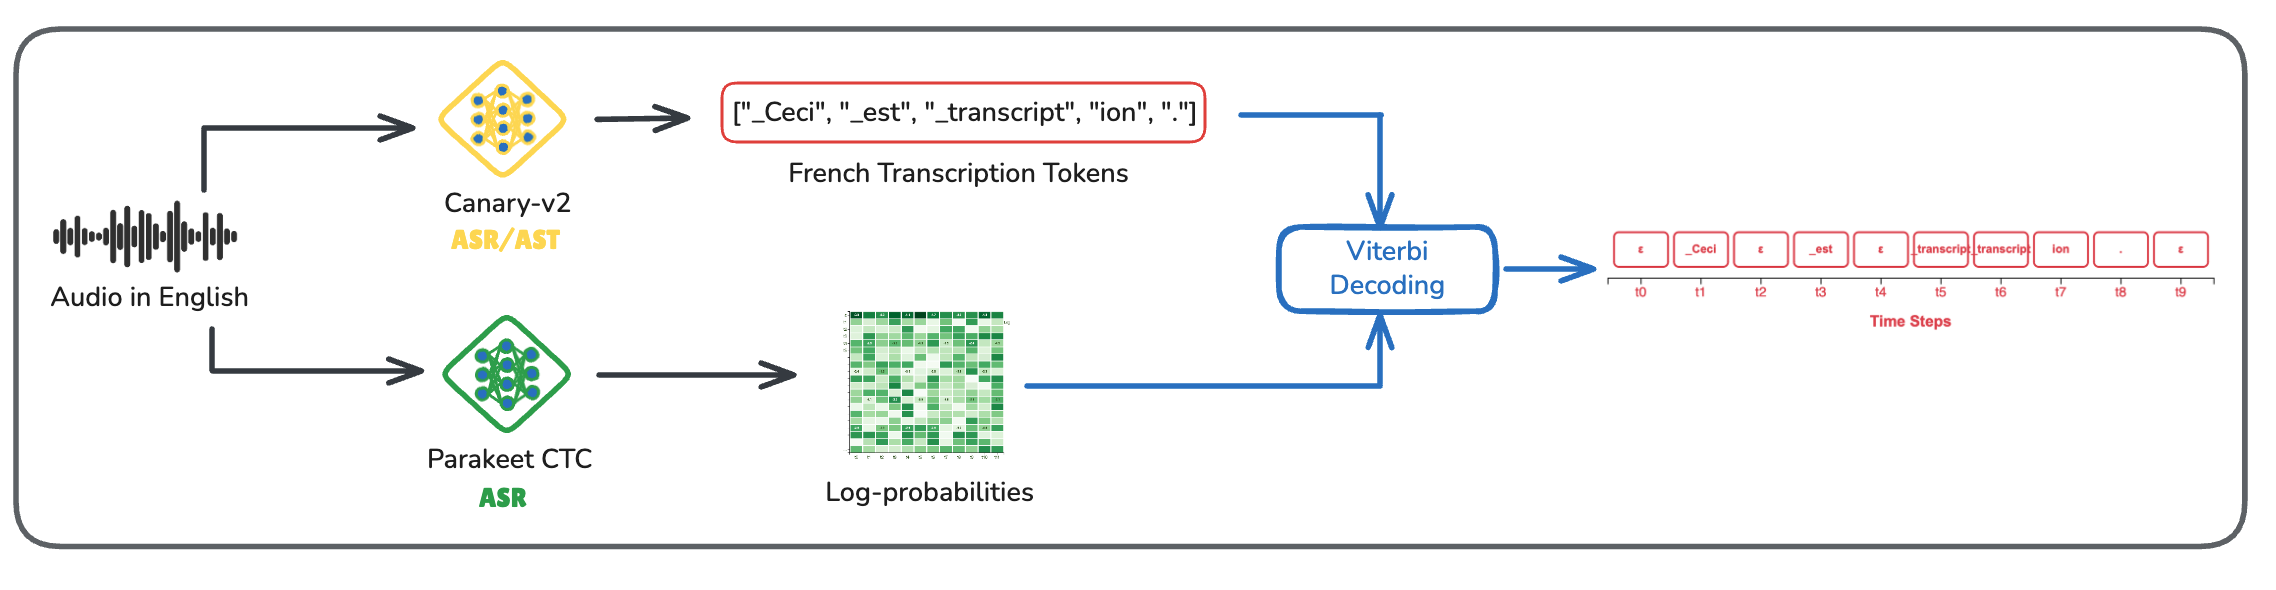
\includegraphics[width=0.95\linewidth]{images/nfa_b.png}
    \caption{Timestamps for AST output.}
    \label{fig:canary-ast}
  \end{subfigure}

  \caption{Overview of Timestamps Generation for Canary-1B-v2 with NFA.}
  \label{fig:canary-timestamps-ast}
\end{figure}


Figure~\ref{fig:canary-timestamps-asr} depicts the timestamp generation process for Canary-1B-v2 speech recognition output using NFA capabilities. This pipeline incorporates an additional ASR model, a Parakeet architecture model with CTC decoder comprising 600M parameters. This model was trained using the same unified tokenizer as Canary-1B-v2 for 250,000 steps on 128 NVIDIA A100 GPUs, using the ASR subset of Canary-1B-v2 training data described in Section~\ref{sec:data}.
When integrating the Forced Alignment pipeline into Canary-1B-v2's inference pipeline, a critical question emerged regarding ASR and AST task alignment: Can NFA effectively align translated speech with audio sequences in completely different languages?

ASR alignment is typically monotonic, maintaining a strictly sequential, left-to-right mapping from temporal audio frames to output phonemes, characters, or words. This "forced alignment" ensures linear correspondence between transcription output and input speech signal.
In contrast, AST alignment is both non-monotonic and cross-lingual. Words and phrases in the source language lack direct, sequential correspondence with translated target language output due to linguistic phenomena including different grammatical structures, verb tenses, and word orders. For example, the English phrase \emph{I love you} translates to French \emph{je t'aime}, where source and target word orders don't align sequentially. 

Additionally, the CTC model (Parakeet CTC) incorporated into the NFA pipeline is trained solely for ASR tasks and lacks AST knowledge.

To evaluate timestamp generation capabilities for AST tasks, we conducted experiments on evaluation benchmarks and performed manual evaluation of the generated timestamps. The NFA pipeline integrated into Canary-1B-v2's inference mechanism successfully produced high-quality segment-level timestamps, as shown in Figure~\ref{fig:canary-timestamps-ast}b. We therefore recommend using segment-level timestamps with translation outputs, as word-level timestamps can be inaccurate due to the non-monotonic nature of speech translation. An example of segment-level timestamps with the respective prompts is illustrated in Figure~\ref{fig:output-examples}. 

Overall, we observed that the current pipeline with NFA yields consistently reliable timestamping performance. We attribute this in part to the fact that our evaluation scope primarily covers European languages, where translations to and from English tend to preserve sentence structure without drastic reordering. By contrast, languages with more divergent syntactic structures such as Mandarin may introduce substantial shifts in word and phrase order. As such, while the results within our explored language set are promising, the applicability of the NFA pipeline to typologically distant languages remains uncertain and warrants more thorough testing and investigation.

\begin{figure}[htbp]
  \centering
  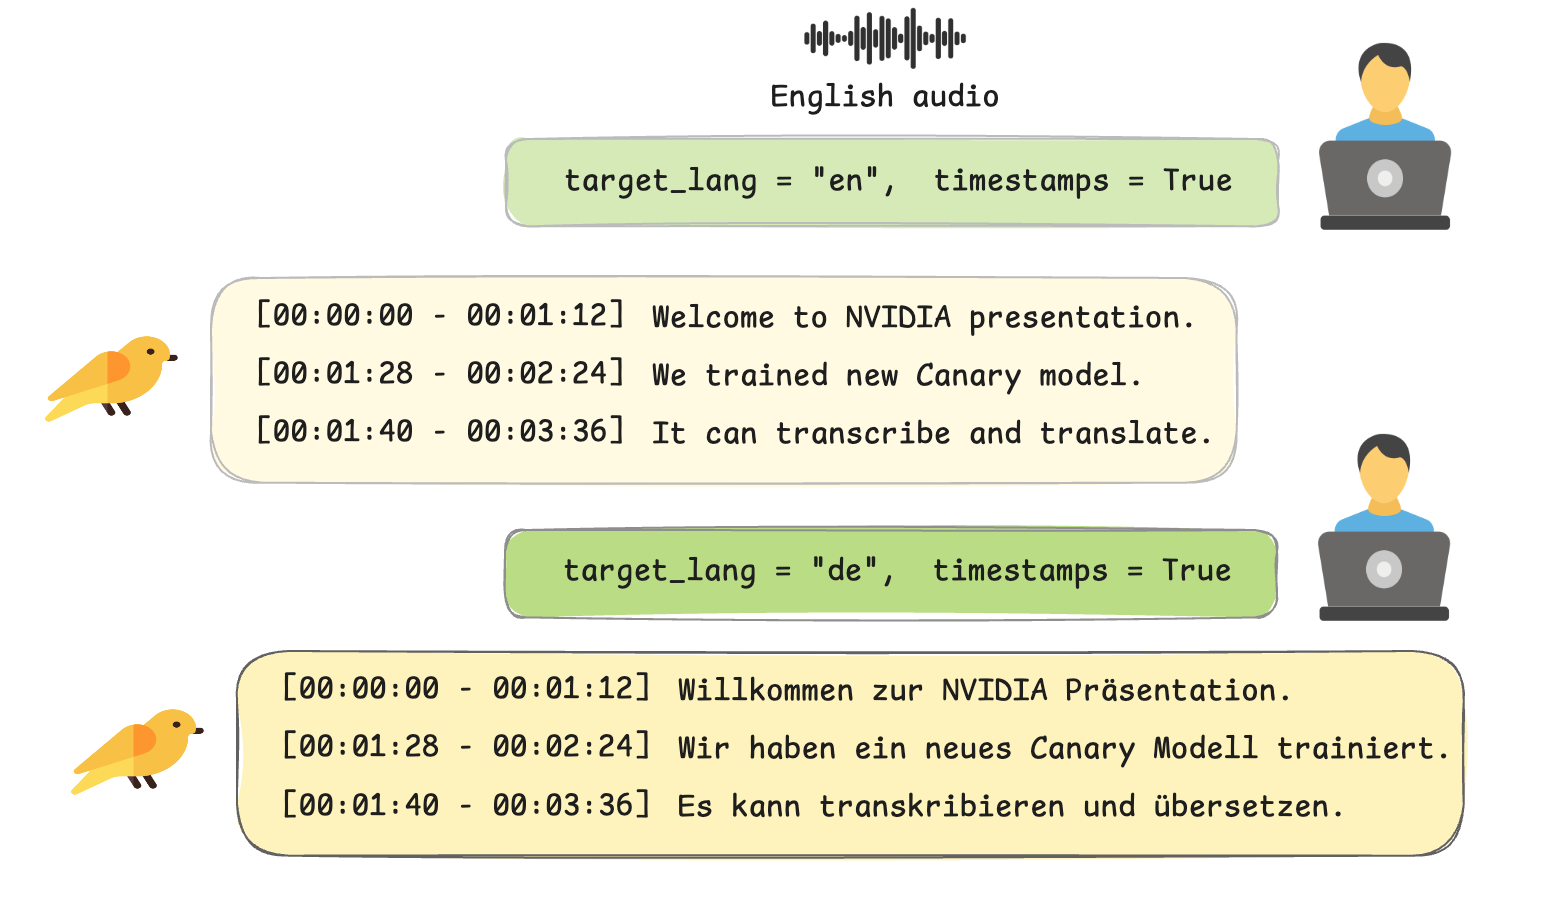
\includegraphics[width=0.6\linewidth]{images/timestamps_example.png}
  \caption{Examples of Canary-1B-v2 output along with segment-level timestamps.}
  \label{fig:output-examples}
\end{figure}

Looking ahead, future work will focus on more comprehensive and quantitative AST timestamp evaluation and on exploring how log-probabilities of an ASR model are effectively leveraged for aligning translation transcript tokens.
